\section{Технологическая часть}

\noindent
\hspace{1.25cm}
В данном разделе проводится анализ систем управления базами данных и выбирается СУБД для решения поставленной задачи, обосновываются средства реализации приложения, приводятся детали реализации базы данных и представляется пример работы программы.

\subsection{Анализ систем управления базами данных}

\noindent
\hspace{1.25cm}
Для хранения истории деформаций трубчатых поверхностей была выбрана реляционная база данных. Были рассмотрены СУБД для работы с ними~\cite{vas_hus}:

\begin{itemize}
    \item \textbf{PostgreSQL} --- объектно-реляционная СУБД с открытым исходным кодом, соответствующая стандартам SQL~\cite{vas_hus}. Обеспечивает строгую типизацию данных, поддержку внешних ключей с каскадными операциями, сложных ограничений целостности (CHECK, UNIQUE), триггеров и хранимых процедур. Поддерживает механизм MVCC (многоверсионное управление конкурентным доступом).
    
    \item \textbf{MySQL} --- реляционная СУБД, разрабатываемая корпорацией Oracle~\cite{mysql}. Имеет ограниченную поддержку механизмов ограничения целостности. Не поддерживает внешние ключи и транзакции. Не соответствует стандартам SQL~\cite{mysql}.
    
    \item \textbf{Oracle Database} --- коммерческая объектно-реляционная СУБД, обеспечивующая безопасность и масштабируемость~\cite{oracle}. Полная функциональность доступна только в платных версиях.
\end{itemize}

\subsubsection{Выбор СУБД для решения задачи}

\noindent
\hspace{1.25cm}
Для выбора оптимальной СУБД были определены критерии сравнения, основанные на требованиях поставленной задачи:

\begin{itemize}
    \item \textbf{К1} --- полная поддержка ACID-транзакций для обеспечения согласованности данных при сохранении версий;
    \item \textbf{К2} --- поддержка внешних ключей с каскадными операциями для автоматического поддержания связей между таблицами;
    \item \textbf{К3} --- поддержка ограничений целостности (CHECK, UNIQUE) для валидации геометрических данных;
    \item \textbf{К4} --- бесплатное использование для академических и коммерческих целей.
\end{itemize}

\noindent
\hspace{1.25cm}
Результаты сравнения СУБД по выбранным критериям приведены в таблице~\ref{tab:dbms_comparison}.

\begin{table}[H]
    \captionsetup{justification=raggedright, singlelinecheck=false}
    \caption{Сравнение СУБД по выбранным критериям}
    \label{tab:dbms_comparison}
    \begin{tabularx}{\textwidth}{|l|>{\centering\arraybackslash}X|>{\centering\arraybackslash}X|>{\centering\arraybackslash}X|>{\centering\arraybackslash}X|}
        \hline
        \textbf{СУБД} & \textbf{К1} & \textbf{К2} & \textbf{К3} & \textbf{К4} \\ \hline
        PostgreSQL & + & + & + & + \\ \hline
        MySQL & $-$ & $-$ & $-$ & + \\ \hline
        Oracle Database & + & + & + & $-$ \\ \hline
    \end{tabularx}
\end{table}

\noindent
\hspace{1.25cm}
По результатам сравнения для решения поставленной задачи выбрана СУБД PostgreSQL.

\subsection{Выбор средств реализации}

\noindent
\hspace{1.25cm}
Для разработки программного обеспечения взаимодействия с базой данных в качестве основного языка программирования был выбран C++~\cite{cpp}. Обоснование выбора:

\begin{itemize}
    \item объектно-ориентированный подход позволяет моделировать иерархию объектов (трубка, сечение, точка);
    \item наличие библиотек для работы с PostgreSQL;
    \item поддержка библиотеки шаблонов для работы с коллекциями данных;
    \item возможность низкоуровневой оптимизации памяти и вычислений.
\end{itemize}

\noindent
\hspace{1.25cm}
Для графического интерфейса используется фреймворк Qt~\cite{qt}, обеспечивающий:
\begin{itemize}
    \item кроссплатформенность разработки;
    \item интеграцию с OpenGL~\cite{opengl} для визуализации трехмерных объектов;
    \item набор виджетов для создания пользовательского интерфейса.
\end{itemize}


\noindent
\hspace{1.25cm}
Для замеров времени использовался класс \texttt{QElapsedTimer} из библиотеки QT~\cite{qt}. Для визуализации трехмерных графиков был использован Python~\cite{python}, а именно библиотека matplotlib~\cite{matplotlib}.


\noindent
\hspace{1.25cm}
Для взаимодействия с базой данных PostgreSQL выбрана библиотека Qt SQL~\cite{qtsql} --- библиотека, предоставляющая:
\begin{itemize}
    \item интерфейс для работы с соединениями и транзакциями;
    \item параметризованные запросы для защиты от SQL-инъекций;
    \item интеграцию с фреймворком Qt;
    \item поддержку подготовленных выражений для повышения производительности.
\end{itemize}

\subsection{Детали реализации}

\subsubsection{Создание таблиц}


\noindent
\hspace{1.25cm}
Создание таблицы \texttt{point} для хранения точек сечений представлено на листинге~\ref{lst:create_point}.

\begin{lstlisting}[caption={Создание таблицы point}, label=lst:create_point, language=SQL]
create table point (
    id bigserial primary key,
    section_id bigint references section(id) on delete cascade,
    ver_id integer not null,
    index_in_section integer,
    x real not null,
    y real not null,
    z real not null,
    future_point_id bigint references point(id) on delete set null,
    past_point_id bigint references point(id) on delete set null,
    constraint unique_point_in_section 
        unique (section_id, index_in_section)
);
\end{lstlisting}

\noindent
\hspace{1.25cm}
Создание таблицы \texttt{section} для хранения сечений трубки представлено на листинге~\ref{lst:create_section}.

\begin{lstlisting}[caption={Создание таблицы section}, label=lst:create_section, language=SQL]
create table section (
    id bigserial primary key,
    tube_id bigint not null references tube(id) on delete cascade,
    ver_id integer not null,
    index integer not null,
    x_cen real not null,
    y_cen real not null,
    z_cen real not null,
    future_section_id bigint references section(id) on delete set null,
    past_section_id bigint references section(id) on delete set null,
    constraint unique_section_in_tube unique (tube_id, index)
);
\end{lstlisting}

\noindent
\hspace{1.25cm}
Создание таблицы \texttt{edge} для хранения ребер между точками представлено на листинге~\ref{lst:create_edge}.

\begin{lstlisting}[caption={Создание таблицы edge}, label=lst:create_edge, language=SQL]
create table edge (
    id bigserial primary key,
    segment_id bigint not null references segment(id) 
        on delete cascade,
    ver_id integer not null,
    index integer not null,
    start_point_id bigint not null references point(id) 
        on delete cascade,
    end_point_id bigint not null references point(id) 
        on delete cascade,
    beg_sz real not null,
    future_edge_id bigint references edge(id) on delete set null,
    past_edge_id bigint references edge(id) on delete set null,
    constraint unique_edge_in_segment unique (segment_id, index),
    constraint different_points 
        check (start_point_id != end_point_id)
);
\end{lstlisting}

\noindent
\hspace{1.25cm}
Создание таблицы \texttt{segment} для хранения сегментов между сечениями представлено на листинге~\ref{lst:create_segment}.

\begin{lstlisting}[caption={Создание таблицы segment}, label=lst:create_segment, language=SQL]
create table segment (
    id bigserial primary key,
    tube_id bigint not null references tube(id) on delete cascade,
    ver_id integer not null,
    index integer not null,
    future_segment_id bigint references segment(id) on delete set null,
    past_segment_id bigint references segment(id) on delete set null,
    constraint unique_segment_in_tube unique (tube_id, index)
);
\end{lstlisting}


\noindent
\hspace{1.25cm}
Создание таблицы \texttt{tube} для хранения информации о трубках представлено на листинге~\ref{lst:create_tube}.

\begin{lstlisting}[caption={Создание таблицы tube}, label=lst:create_tube, language=SQL]
create table tube (
    id bigserial primary key,
    ver_id integer not null,
    len real not null,
    future_tube_id bigint references tube(id) on delete set null,
    past_tube_id bigint references tube(id) on delete set null
);
\end{lstlisting}

\subsubsection{Хранимые процедуры и функции}

\noindent
\hspace{1.25cm}
Создание функции для пересчета длины трубки при изменениях в \texttt{segment}~\ref{lst:create_f_seg}.

\begin{lstlisting}[caption={Функция для пересчета длины трубки при изменениях в \texttt{segment}}, label=lst:create_f_seg, language=SQL]
create or replace function calculate_tube_length_on_segment()
returns trigger as $$
declare
    tube_id_val bigint;
    new_length real;
    current_length real;
begin
    if tg_op = 'DELETE' then
        tube_id_val := old.tube_id;
    else
        tube_id_val := new.tube_id;
    end if;

    select coalesce(sum(max_edge_length), 0) into new_length
    from (
        select s.id, max(e.beg_sz) as max_edge_length
        from segment s
        left join edge e on e.segment_id = s.id
        where s.tube_id = tube_id_val
        group by s.id
    ) as segment_lengths;
    
    select len into current_length
    from tube
    where id = tube_id_val;

    if current_length is distinct from new_length then
        update tube
        set len = new_length
        where id = tube_id_val;
    end if;

    if tg_op = 'DELETE' then
        return old;
    else
        return new;
    end if;
end;
$$ language plpgsql;
\end{lstlisting}

\noindent
\hspace{1.25cm}
Создание функции для пересчета длины трубки при изменениях в \texttt{edge}~\ref{lst:create_f_edge}.

\begin{lstlisting}[caption={Функция для пересчета длины трубки при изменениях в \texttt{edge}}, label=lst:create_f_edge, language=SQL]
create or replace function calculate_tube_length_on_edge()
returns trigger as $$
declare
    tube_id_val bigint;
    new_length real;
    current_length real;
begin
    if tg_op = 'DELETE' then
        select tube_id into tube_id_val
        from segment
        where id = old.segment_id;
    else
        select tube_id into tube_id_val
        from segment
        where id = new.segment_id;
    end if;

    select coalesce(sum(max_edge_length), 0) into new_length
    from (
        select s.id, max(e.beg_sz) as max_edge_length
        from segment s
        left join edge e on e.segment_id = s.id
        where s.tube_id = tube_id_val
        group by s.id
    ) as segment_lengths;

    select len into current_length
    from tube
    where id = tube_id_val;

    if current_length is distinct from new_length then
        update tube
        set len = new_length
        where id = tube_id_val;
    end if;

    if tg_op = 'DELETE' then
        return old;
    else
        return new;
    end if;
end;
$$ language plpgsql;
\end{lstlisting}

\subsubsection{Триггеры базы данных}

\noindent
\hspace{1.25cm}
Создание триггера для пересчета длины трубки при изменениях в \texttt{segment}~\ref{lst:create_trigger_seg}.

\begin{lstlisting}[caption={Триггер для пересчета длины трубки при изменениях в \texttt{segment}}, label=lst:create_trigger_seg, language=SQL]
create trigger update_tube_length_on_segment
after insert or update or delete on segment
for each row
execute function calculate_tube_length_on_segment();
\end{lstlisting}

\noindent
\hspace{1.25cm}
Создание триггера для пересчета длины трубки при изменениях в \texttt{edge}~\ref{lst:create_trigger_edge}.

\begin{lstlisting}[caption={Триггер для пересчета длины трубки при изменениях в \texttt{edge}}, label=lst:create_trigger_edge, language=SQL]
create trigger update_tube_length_on_edge
after insert or update of beg_sz or delete on edge
for each row
execute function calculate_tube_length_on_edge();
\end{lstlisting}


\subsection{Пример работы программы}

\noindent
\hspace{1.25cm}
Интерфейс программы включает следующие основные элементы:
\begin{itemize}
    \item главное окно с трехмерным просмотром трубки;
    \item панель управления сечениями;
    \item панель настройки параметров деформации;
    \item панель истории версий с навигацией;
    \item диалоговые окна для сохранения и загрузки данных.
\end{itemize}

\noindent
\hspace{1.25cm}
Разработанное программное обеспечение предоставляет следующий функционал:

\begin{enumerate}
    \item \textbf{Создание и сохранение трубки:}
    \begin{itemize}
        \item построение трубчатой поверхности на основе заданных сечений;
        \item сохранение геометрии трубки в базу данных с присвоением версии;
        \item автоматическое сохранение всех сечений, точек, сегментов и ребер.
    \end{itemize}
    
    \item \textbf{Применение деформации:}
    \begin{itemize}
        \item выбор точки деформации на кривой центров трубки (рисунок~~\ref{fig:ui_1});
        
        
\begin{figure}[H]
\centering
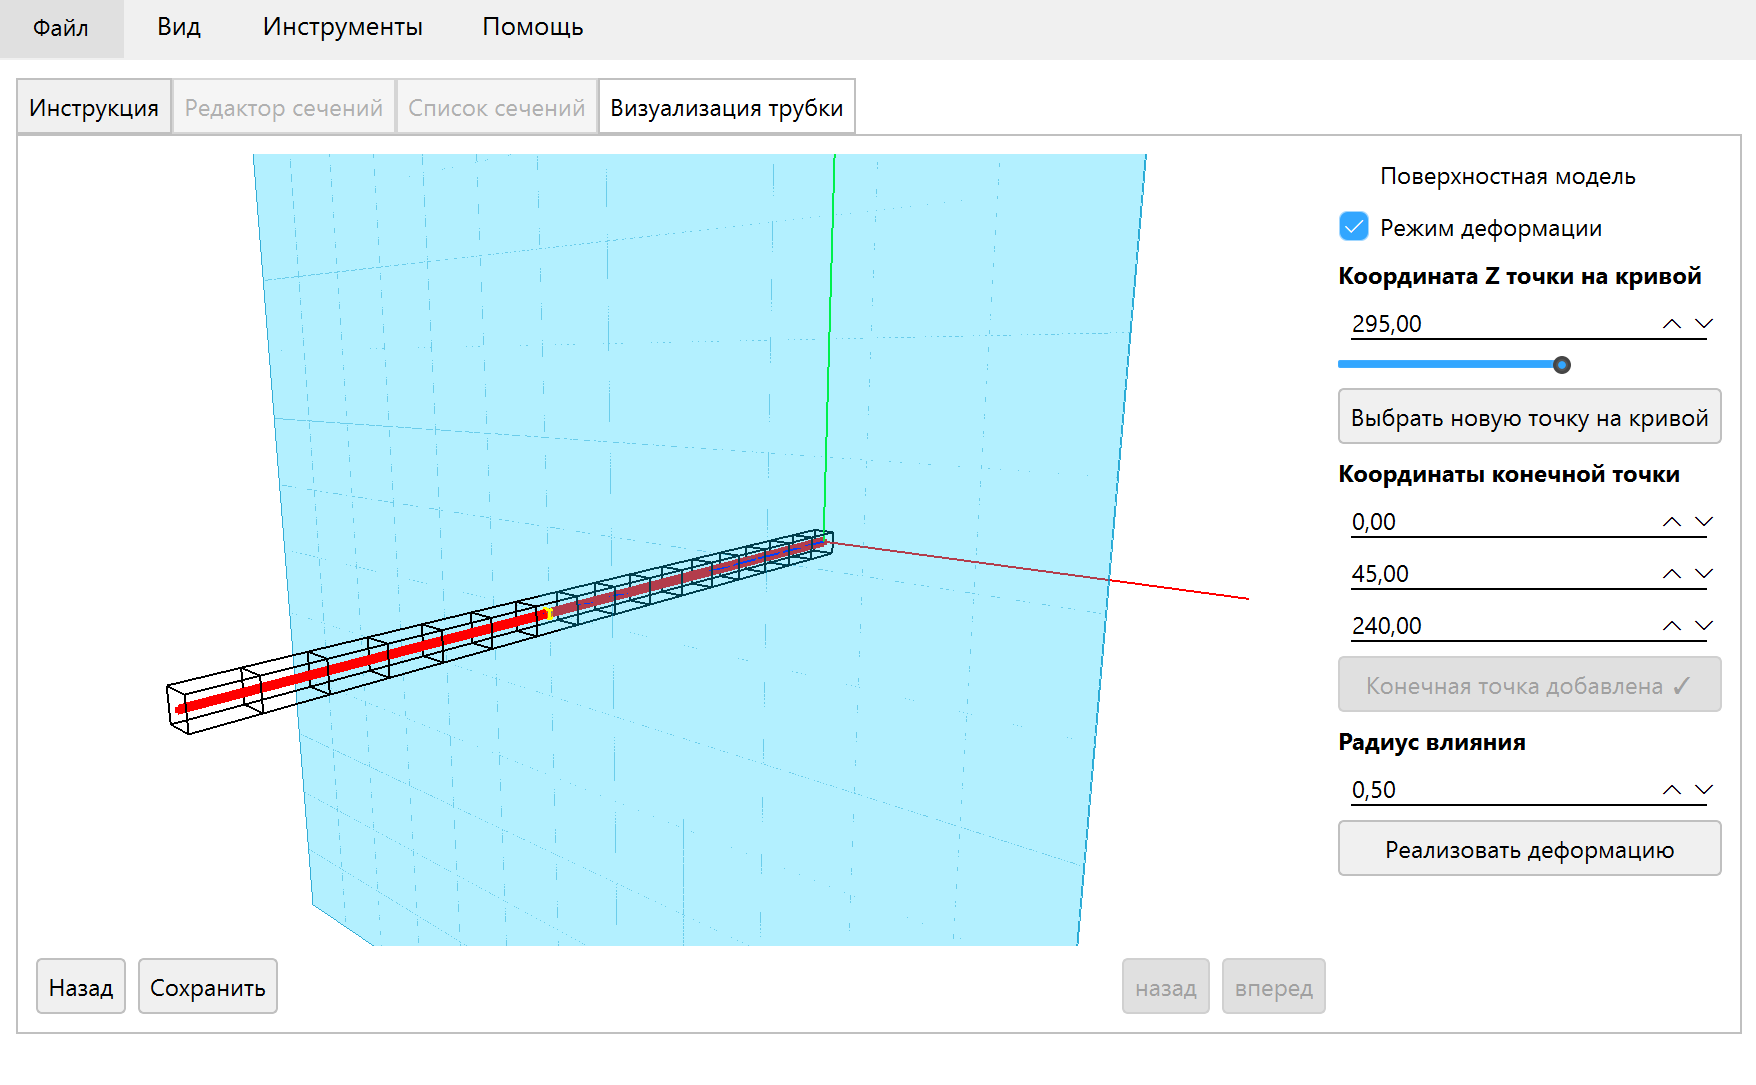
\includegraphics[width=1.0\textwidth]{img/ui_1.png}
\caption{Выбор точки деформации}
\label{fig:ui_1}
\end{figure}


        \item указание целевой позиции для перемещения выбранной точки;
        \item настройка радиуса влияния и функции затухания деформации;
        \item визуализация деформированной кривой центров в режиме предварительного просмотра (рисунок~\ref{fig:ui_2});
        
               
\begin{figure}[H]
\centering
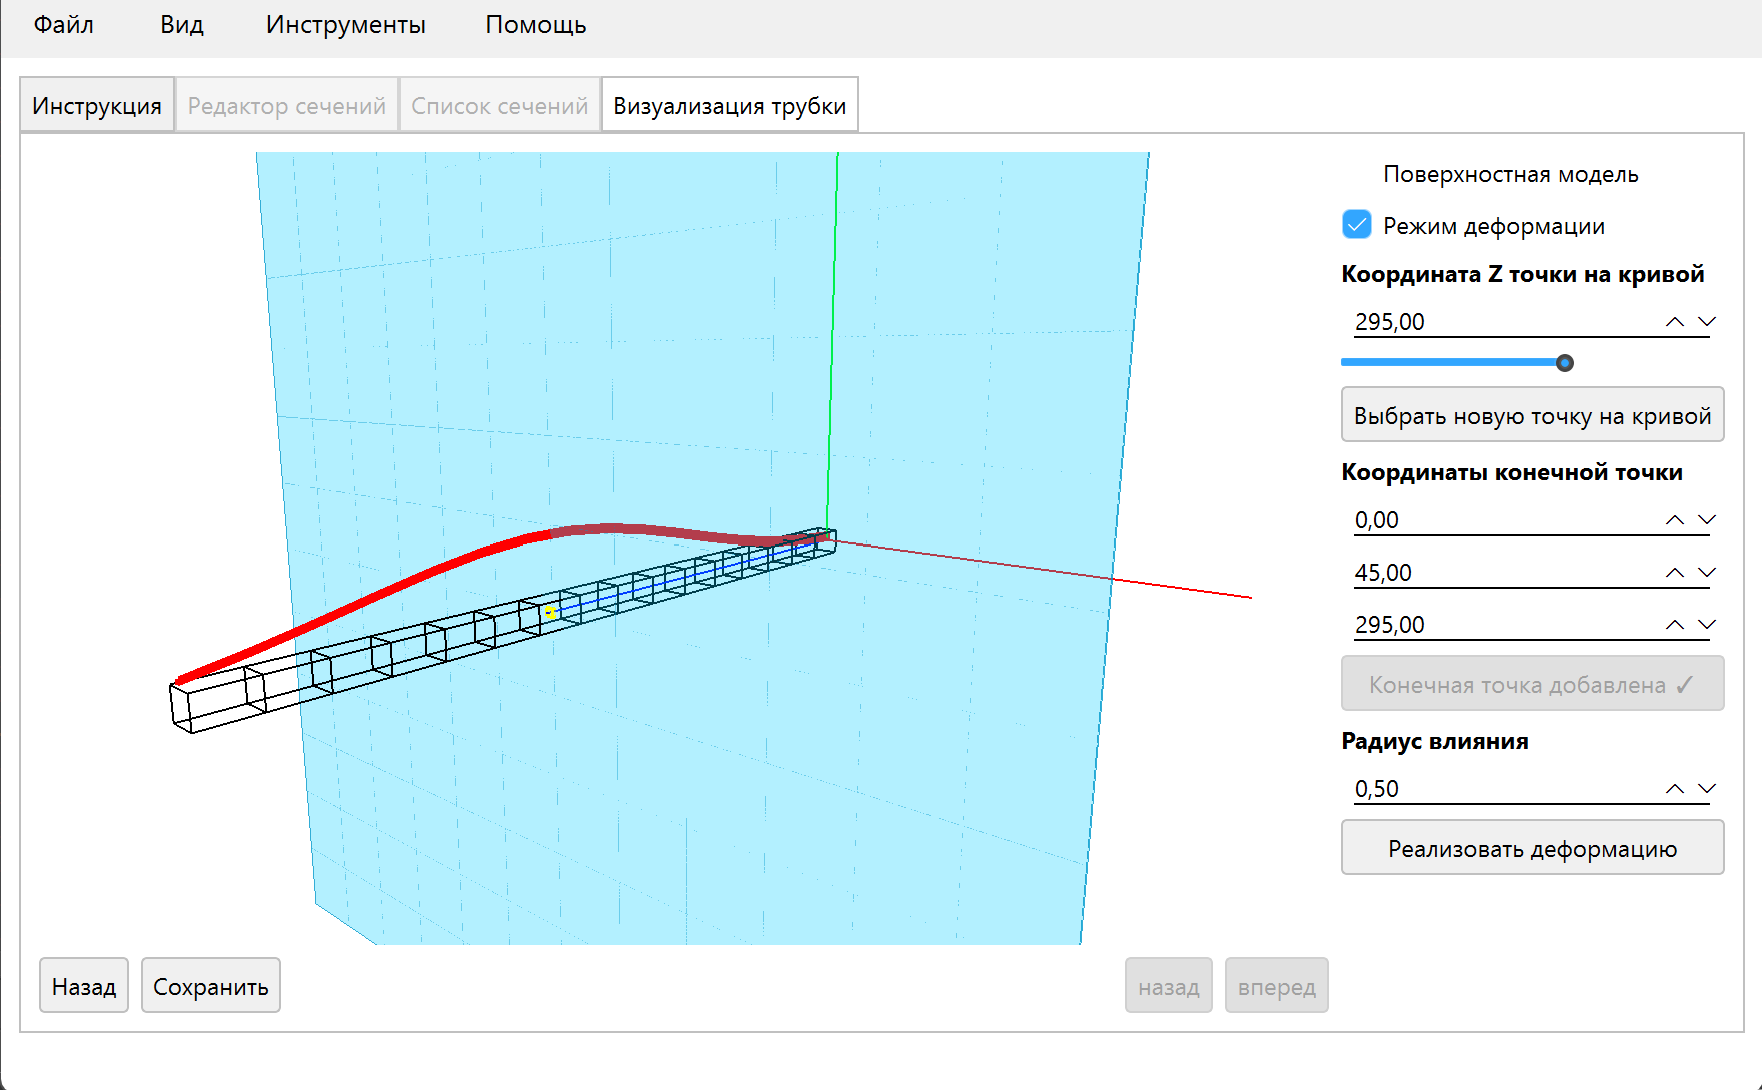
\includegraphics[width=1.0\textwidth]{img/ui_2.png}
\caption{Визуализация деформированной кривой центров}
\label{fig:ui_2}
\end{figure}


        \item применение деформации с автоматическим пересчетом геометрии (рисунок~~\ref{fig:ui_3}).
        
               
\begin{figure}[H]
\centering
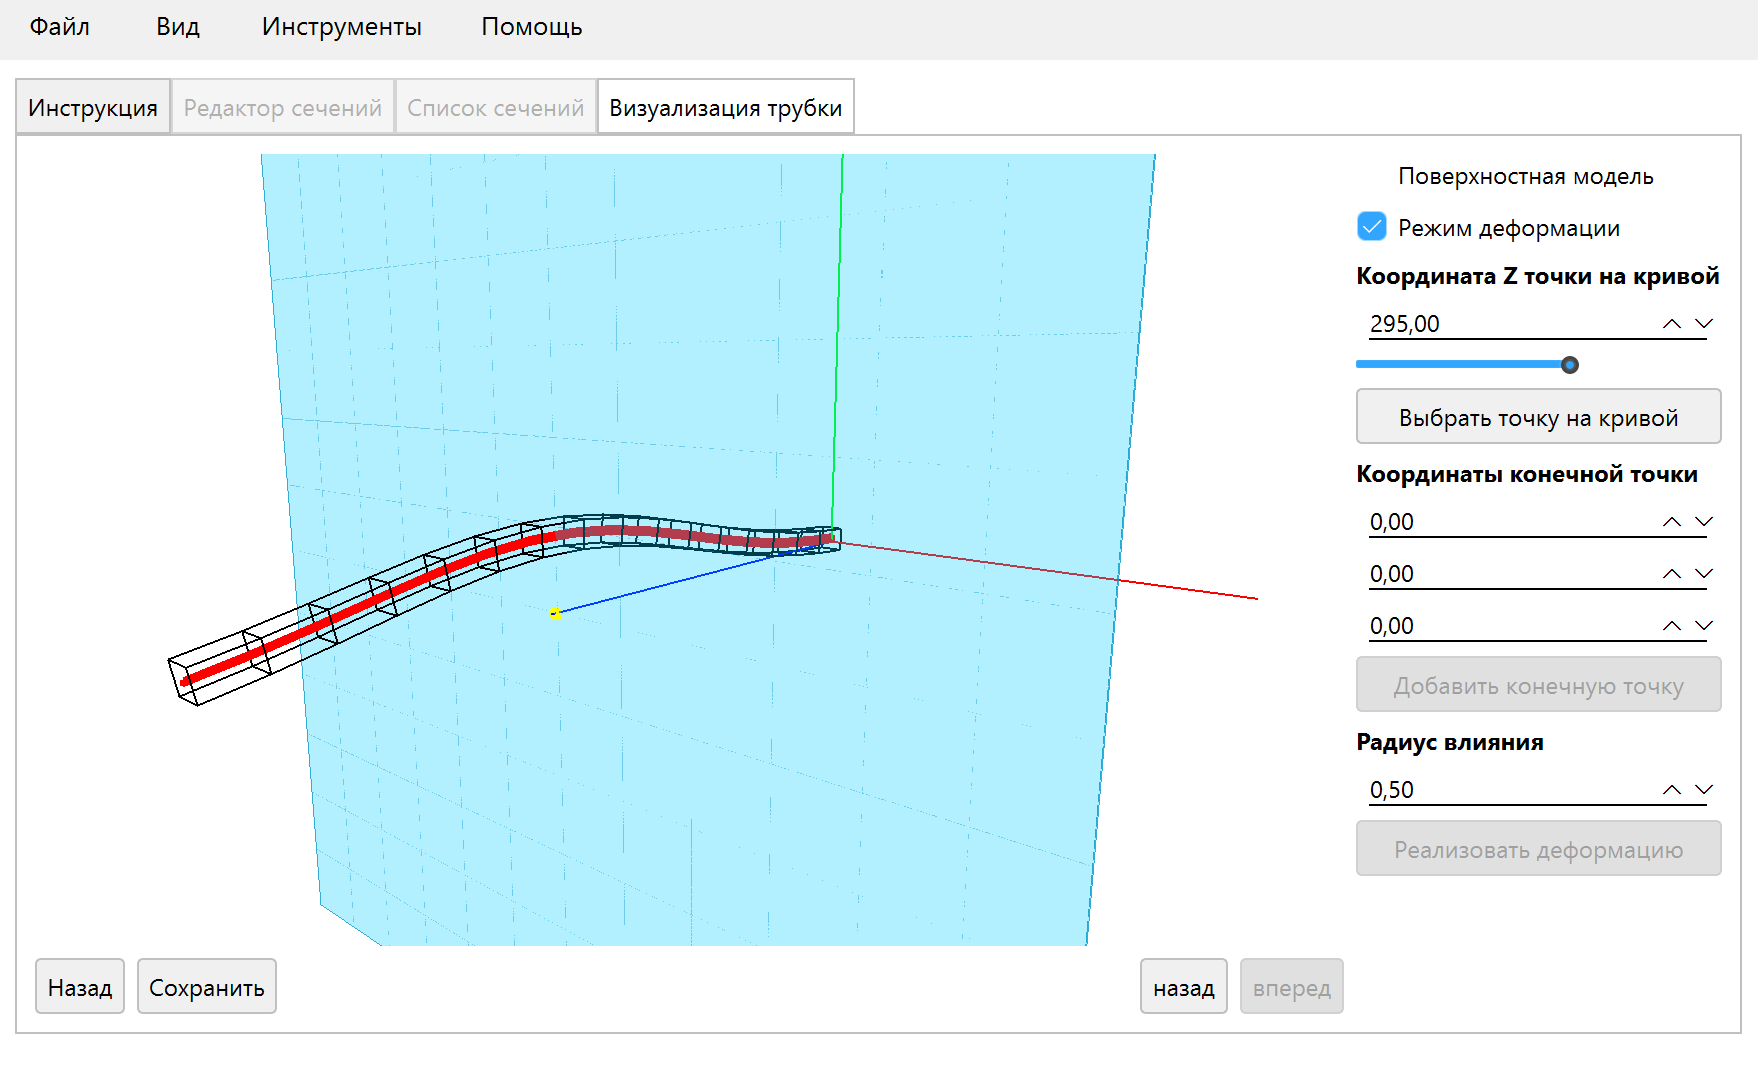
\includegraphics[width=1.0\textwidth]{img/ui_3.png}
\caption{Применение деформации}
\label{fig:ui_3}
\end{figure}


    \end{itemize}
    
    \item \textbf{Просмотр истории изменений.}
    
    
   
\end{enumerate}

\subsection{Вывод}


\noindent
\hspace{1.25cm}
В данном разделе проведен анализ систем управления базами данных, в результате которого для решения поставленной задачи выбрана СУБД PostgreSQL, обоснован выбор языка программирования C++ и библиотеки Qt SQL для взаимодействия с базой данных, приведены детали реализации и представлен пример работы программы.

\newpage